% A simple LaTeX template for lab reports in TDT4258 Energy Efficient Computer Design
% by Yaman Umuroglu (yamanu@idi.ntnu.no)
% Feel free to customize the style as you see fit, but the chapters/sections mentioned in the
% template should be included with the appropriate content.

\documentclass[abstract=on]{article}
\textwidth 6in
\oddsidemargin 0.2in
\usepackage[utf8]{inputenc}
\usepackage{tabto}
\usepackage{datetime}
\usepackage{pgfmath}
\usepackage{lipsum}
\usepackage{hyperref}

\usepackage[T1]{fontenc}
\usepackage{textcomp}
\usepackage{gensymb}

\usepackage{natbib}
\usepackage{graphicx}
\usepackage[norsk]{babel}
\usepackage{listings}
\usepackage{color}
\usepackage[table]{xcolor}
\usepackage{tabularx}
\usepackage{multirow}

 
% "define" Scala
\lstdefinelanguage{scala}{
  morekeywords={abstract,case,catch,class,def,%
    do,else,extends,false,final,finally,%
    for,if,implicit,import,match,mixin,%
    new,null,object,override,package,%
    private,protected,requires,return,sealed,%
    super,this,throw,trait,true,try,%
    type,val,var,while,with,yield},
  otherkeywords={=>,<-,<\%,<:,>:,\#,@},
  sensitive=true,
  morecomment=[l]{//},
  morecomment=[n]{/*}{*/},
  morestring=[b]",
  morestring=[b]',
  morestring=[b]"""
}

\definecolor{dkgreen}{rgb}{0,0.6,0}
\definecolor{gray}{rgb}{0.5,0.5,0.5}
\definecolor{mauve}{rgb}{0.58,0,0.82}
 
% Default settings for code listings
\lstset{frame=tb,
  language=scala,
  aboveskip=3mm,
  belowskip=3mm,
  showstringspaces=false,
  columns=flexible,
  basicstyle={\small\ttfamily},
  numbers=none,
  numberstyle=\tiny\color{gray},
  keywordstyle=\color{blue},
  commentstyle=\color{dkgreen},
  stringstyle=\color{mauve},
  frame=single,
  breaklines=true,
  breakatwhitespace=true
  tabsize=3
}

%\lstdefinestyle{customc}{
%  belowcaptionskip=1\baselineskip,
%  breaklines=true,
%  frame=L,
%  xleftmargin=\parindent,
%  language=Scala,
%  showstringspaces=false,
%  basicstyle=\footnotesize\ttfamily,
%  keywordstyle=\bfseries\color{green!40!black},
%  commentstyle=\itshape\color{purple!40!black},
%  identifierstyle=\color{blue},
%  stringstyle=\color{orange},
%}

\newcommand{\mytitle}{Big Data Project}
\newcommand{\mygroupnumber}{64}
\newcommand{\myauthor}{Christoffer Viken\\Ilse Gerda Visser}

\title{\mytitle}
\author{\myauthor}
\date{\today}

\begin{document}


\begin{titlepage}
%\includegraphics[height=1.5cm]{images/ntnu_logo.pdf}\\[1cm]   
\begin{center}

 
% Upper part of the page
~\\[1.5cm]

\textsc{\Large TDT4305\\Big Data}\\[0.5cm]

% Set the title of the Document between two horizontal lines
\hrule ~\\[0.2cm]
{\huge \bfseries \mytitle}\\[0.4cm]   % print the title of the document
\hrule ~\\[1.5cm]

% Additional Information about the document
\begin{minipage}{0.4\textwidth}
    \centering
  \large
    \emph{Group \mygroupnumber:}\\~\\
    \myauthor
\end{minipage}

\vfill

% Bottom of the page
{\large \today}
\end{center}
\end{titlepage}




\section{Exploratory Analysis of Foursquare Dataset}
Several steps were required in order to make 

\subsection{Loading the dataset}
\begin{lstlisting}
var fsData = sc.textFile(file, 2)
//Now we need to get rid of the header line
val allOfIt = fsData
val header = allOfIt.first
fsData = fsData.filter(_ != header).map(x => x.split("\t"))
\end{lstlisting}

\subsection{Calculate the local time}
So obviously we need to convert it from a string to something where we can apply date math.
\begin{lstlisting}
def getLocalTime(utcString: String, localOffset: Int): LocalDateTime = {
    val dateFormat = DateTimeFormatter.ofPattern("yyyy-MM-dd HH:mm:ss", Locale.ENGLISH)
    val utcTime = LocalDateTime.parse(utcString, dateFormat)
    utcTime.plusMinutes(localOffset)
}
\end{lstlisting}

\subsection{Assign a country and city}
\begin{lstlisting}
val cities = buildKDTree(sc.textFile(cities_file, 2).map(line => new City(line)).collect())

def closestCity(lon: Double, lat: Double): City = {
    cities.findNearestNode(lon, lat)
}
\end{lstlisting}

\subsection{Generate a base RDD with a minimal tuple}
\begin{lstlisting}
val dataSet = allOfIt.map(line => {
    val data = line.split("\t")

    (data(1).toInt, //uID _1
      data(2), //sID _2
      getLocalTime(data(3), data(4).toInt), //Time _3
      data(5).toDouble, //lat _4
      data(6).toDouble, //lon _5
      data(7) //cat _6
    )

    }).persist(StorageLevel.MEMORY_AND_DISK)
\end{lstlisting}

\subsection{Answers to questions about numbers}
\subsubsection{Total number of unique users}
\begin{lstlisting}
print("Users: ")
println(dataSet.map(ci => ci._1).distinct.count()) // 256307
\end{lstlisting}

\subsubsection{Number of check-ins}
\begin{lstlisting}
print("Total: ")
println(dataSet.count()) // 19265256
\end{lstlisting}

\subsubsection{Number of check-in sessions}
\begin{lstlisting}
print("Sessions: ") 
println(dataSet.map(ci => ci._2).distinct.count()) // 6338302
\end{lstlisting}

\subsubsection{Number of countries}
\begin{lstlisting}
print("Countries: ")
println(citiesSet.map(ci => ci._1).distinct.count()) // 77
\end{lstlisting}

\subsubsection{Number of cities}
\begin{lstlisting}
print("Cities: ")
println(citiesSet.count()) // 414
\end{lstlisting}



\subsection{Preparing for more analysis}
Now we need to condense down the analysis, so we make key-value pairs and aggregate with those keys
\begin{lstlisting}
val sessions = dataSet
  .map(x => (x._2, Array[(Double, Double, LocalDateTime, String, String)]((x._4, x._5, x._3, x._6, x._2))))
  .aggregateByKey(Array[(Double, Double, LocalDateTime, String, String)]())((k, v) => v ++ k, (v, k) => k ++ v)
  .values.cache()
\end{lstlisting}
Because we are going to use this a couple of times (2) we need to remind spark of that.
We threw away the session key, but store it for every instance in the list.


\subsection{Calculate number of check-ins per session}
The histogram gets calculated and output.
This is simply by using the checkin-count as key and 1 as value, then reduce, and print the resulting values.
\begin{lstlisting}
sessions.map(x => (x.length, 1)).reduceByKey((n1, n2) => n1+n2).saveAsTextFile(out_file + "_histogram")
\end{lstlisting}

\begin{center}
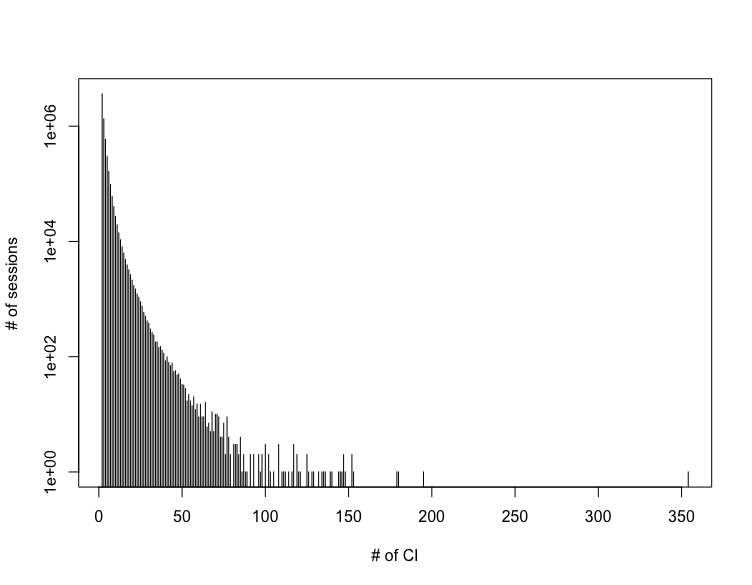
\includegraphics[width=0.8\textwidth]{log-hist.png}\\
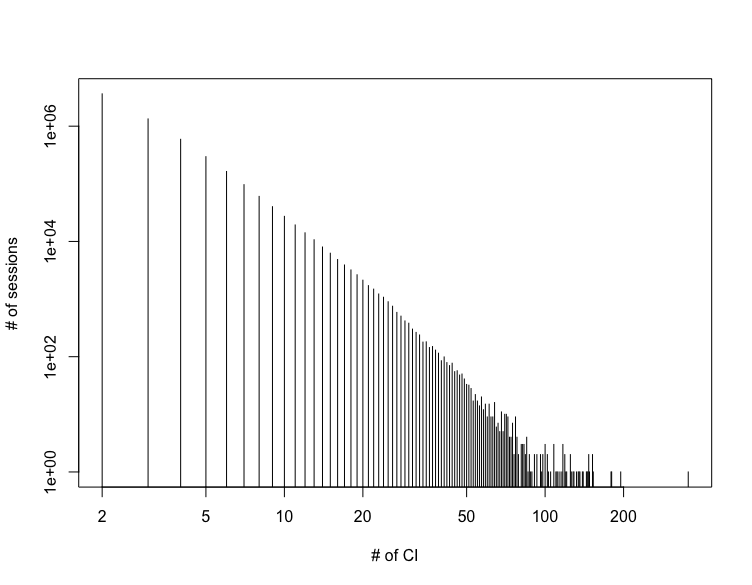
\includegraphics[width=0.8\textwidth]{log_log_hist.png}
\end{center}
% TODO: Picture of histogram here


\subsection{Calculate the distance of session with 4 or more check-ins}
Filter on number of checkins.
Perform a length check for each session. (remember to sort it first, because A->B->C != A->C->B)
Use length as key, we don't have a wrapping type, so tuple (length, checkins) will do.
\begin{lstlisting}
val sessions2 = sessions
  .filter(sess => sess.length > 4)
  .map(ci => {
      //I don't care about reverse order. A session is just as long backwards, but the order needs to be correct.
      ci.sortWith((x, y) => x._3.compareTo(y._3) > 0)
      var length = 0.0
      for (i <- 1 until ci.length) {
        val a = ci(i)
        val b = ci(i - 1)
        length = length + distance_between(a._1, a._2, b._1, b._2)
      }
      (length, ci)
  }
)
\end{lstlisting}

\subsection{Find the 100 longest sessions, covering at least 50 km}
First, filter on session length. We don't want to shuffle around all the values, just the ones with a distance > 50km.
Serialize the session to a TSV string
Second, get 100 sessions using takeOrdered (it sorts and gets the sessions)
\begin{lstlisting}
val sess_strings = sessions2.mapValues(x => x.map(y => {
  y._1 + "\t" + y._2 + "\t" + y._3 + "\t" + y._4 + "\t" + y._5
}))
  .filter(x => x._1 > 50.0)
  .takeOrdered(100)(Ordering[Double].on(x => -x._1))
.map(x => x._2.mkString("\n")) //.mkString("\n")
\end{lstlisting}
At this point we have a regular array and manually output it to a file.


\subsection{Visualize the longest sessions in CartoDB}
Published at:
\url{https://cvi.cartodb.com/viz/93da5988-fd7f-11e5-8456-0ea31932ec1d/public_map}
\begin{center}
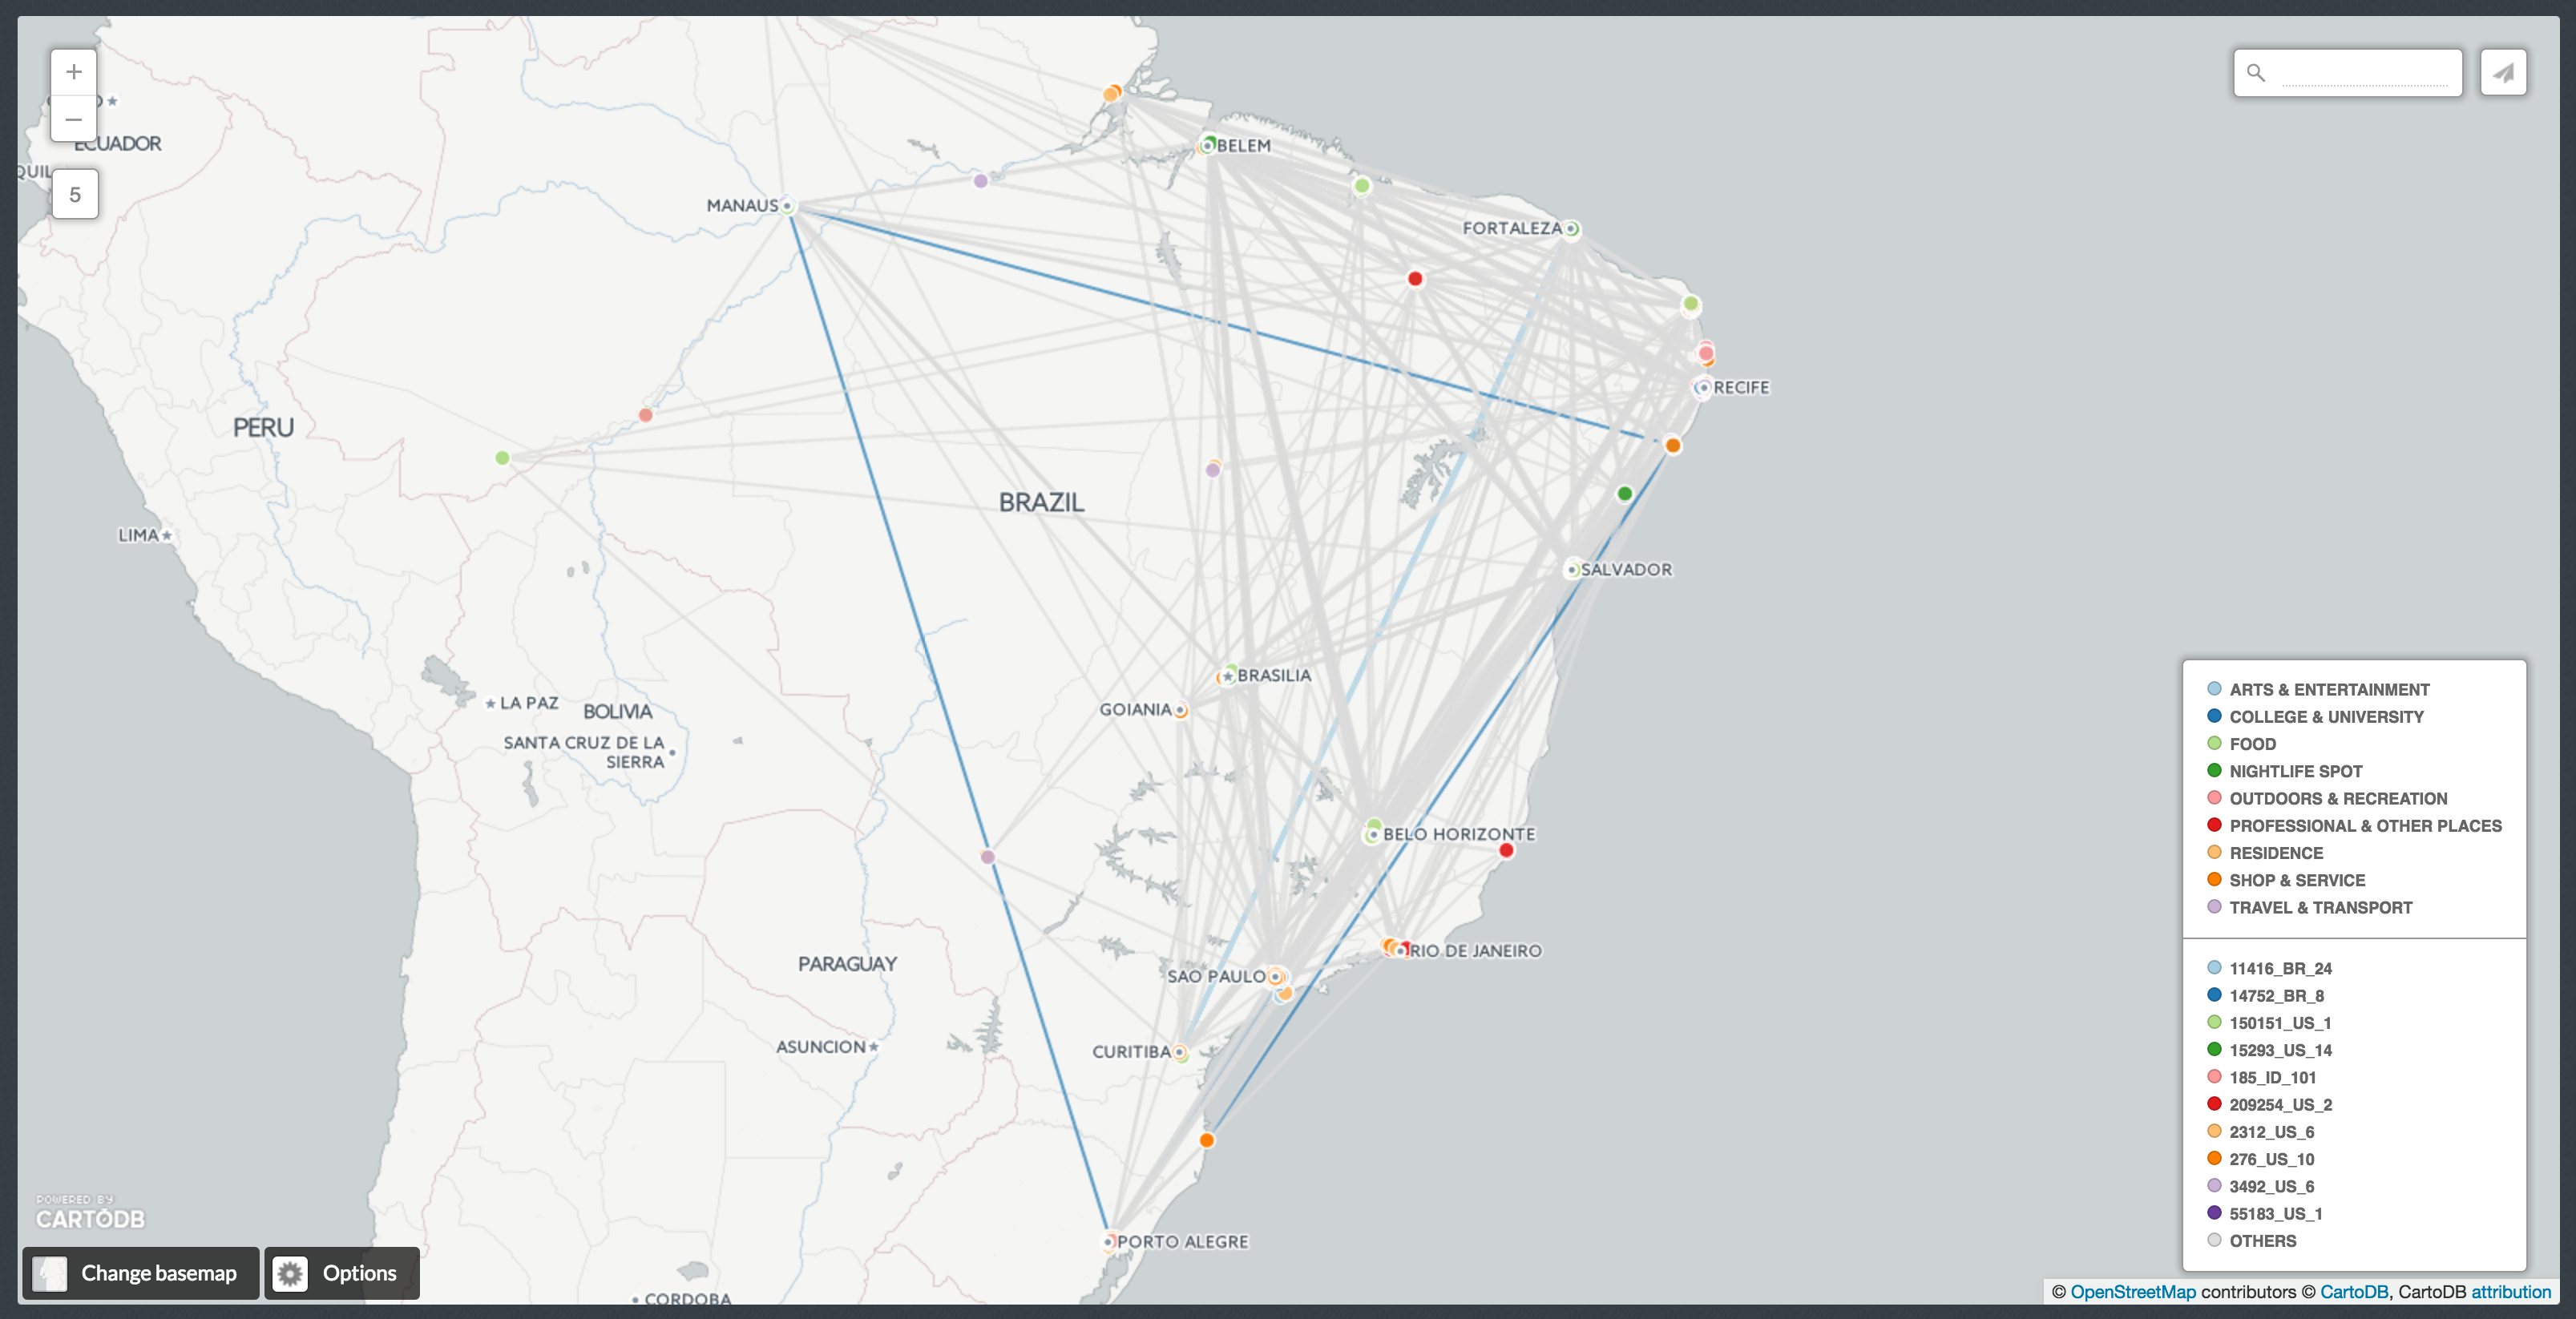
\includegraphics[width=0.8\textwidth]{carto.png}
\end{center}

Query used to extract paths (assuming tabe is named out3):
\begin{lstlisting}[language=SQL]
SELECT
    sess,
    ST_MakeLine(
        ARRAY(SELECT the_geom FROM out3 WHERE o3.sess = out3.sess ORDER BY DATE ASC)
    ) AS the_geom_webmercator
FROM out3 AS o3 GROUP BY sess
\end{lstlisting}

\section{Spark methods used}

\begin{center}
\begin{tabularx}{0.75\textwidth}{ |X| }
\hline
\cellcolor[gray]{0.9}
RDD.filter() \\ \hline
Filter takes a function as an argument (lambda), this function returns true 
if the record is to remain in the RDD otherwise it is removed form the RDD. 
\\ \hline
\hline
\cellcolor[gray]{0.9}
RDD.map() \\ \hline
For each record in the RDD apply the passed function to it, the output is the 
 new record.
\\ \hline
\hline
\cellcolor[gray]{0.9}
RDD.persist() \\ \hline
Keep this RDD, because it may come in handy later on.
\\ \hline
\hline
\cellcolor[gray]{0.9}
RDD.unpersist() \\ \hline
There is little chance of this RDD becoming handy after this point, so throw it 
away.
\\ \hline
\hline
\cellcolor[gray]{0.9}
RDD.cache() \\ \hline
Same as persist, but does not bother with saving to disk.
\\ \hline
\hline
\cellcolor[gray]{0.9}
RDD.reduceByKey() \\ \hline
When applied to a key-value-pair RDD this function will join the functions with 
the same key together using the passed
function.
\\ \hline
\hline
\cellcolor[gray]{0.9}
RDD.aggregateByKey()() \\ \hline
Works as reduceByKey, but takes: an initial value, a partition-reducer and a 
cross-partition-reducer. The partition-reducer is a function that reduces 
records internal to a partition, thus reducing the number of records that need 
to be shuffled later on. The cross-partition-reducer reduces the records after 
the partition-shuffle.
\\ \hline

\hline
\cellcolor[gray]{0.9}
RDD.distinct() \\ \hline
Removes duplicates from the dataset.
\\ \hline
\end{tabularx}

\end{center}
aggregateByKey() have an advantage if the data can be significantly reduced internally to a partition.

\end{document}
